\chapter{Implementation}

\section{App}
Nordic Semi Conductors, the maker of the used microcontrolers, published the code to a simple app that allows for BLE communication with their devices.
It is called nRF Toolbox.
It is intended to pair with the ble\_ app\_ uart example, published in the nRF52 SDK.
Since this example code was used as the basis for the ble communication used in this project, it was addapted to work with this project.


The App contains different modules, intended for different examples, among them the Universal Asynchronus Receiver/Transmitter (UART) module (see \ref{f:Toolbox_modules}).
It is intended to be used with the ble\_ app\_ uart example.
When opem it shows the ble services that are currently beeing addvertised and allows the user to connect to one of them \ref{f:Toolbox_connect}.
It then opens a window similar to phone messangers, were the keyboard can be used to tpye messages, that are sent to the connected devices.

\begin{figure}[ht!]
\centering
 \caption{nRF Toolbox module menue, with the added Art Tracking Module}
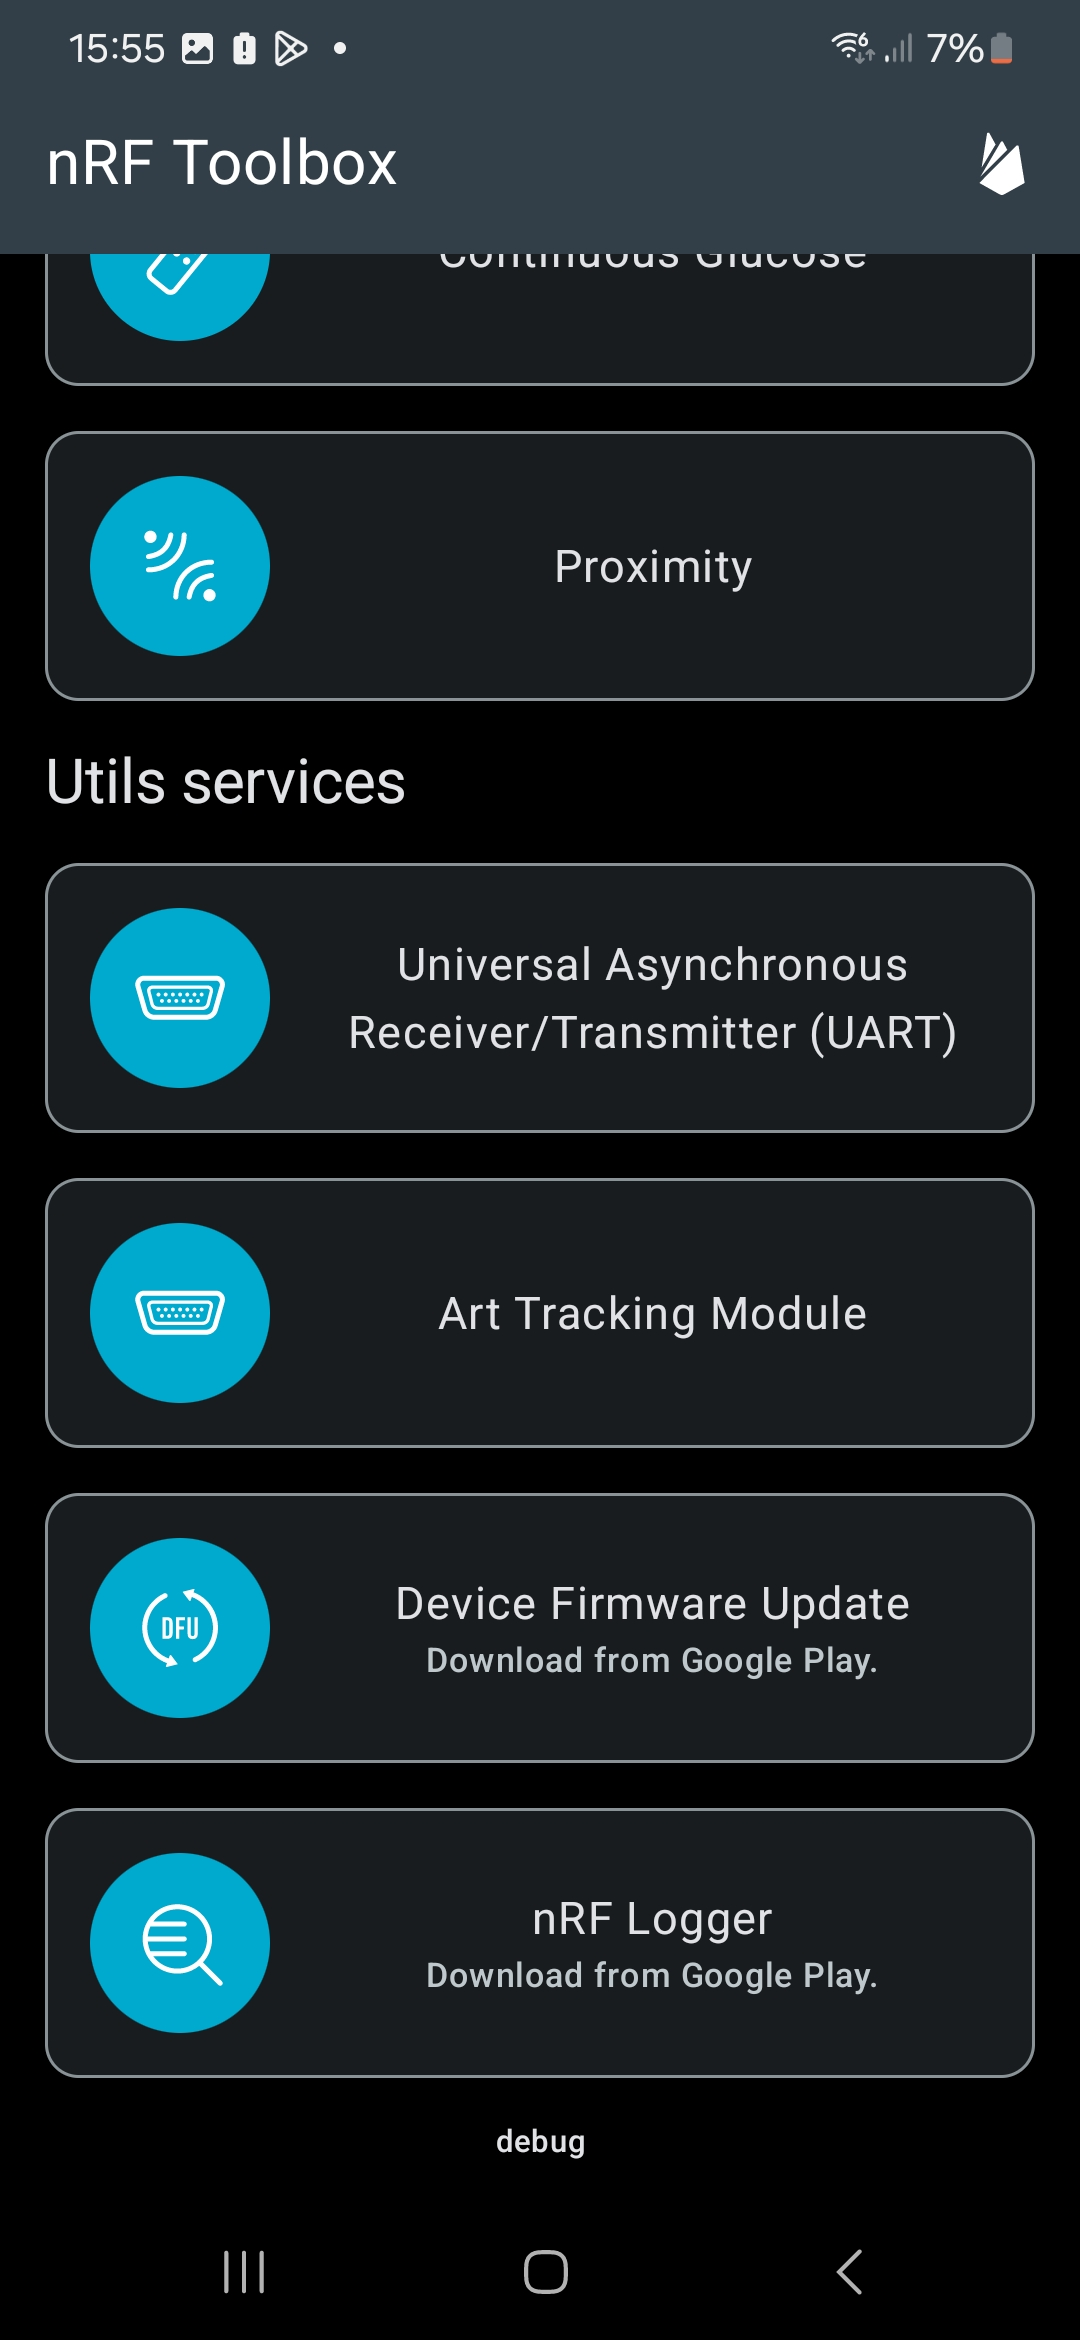
\includegraphics[width=200px]{graphics/nRF_toolbox_modules.jpg}
\label{f:Toolbox_modules}
\end{figure}

\begin{figure}[ht!]
\centering
 \caption{nRF Toolbox shows avaliable devices to connect to}
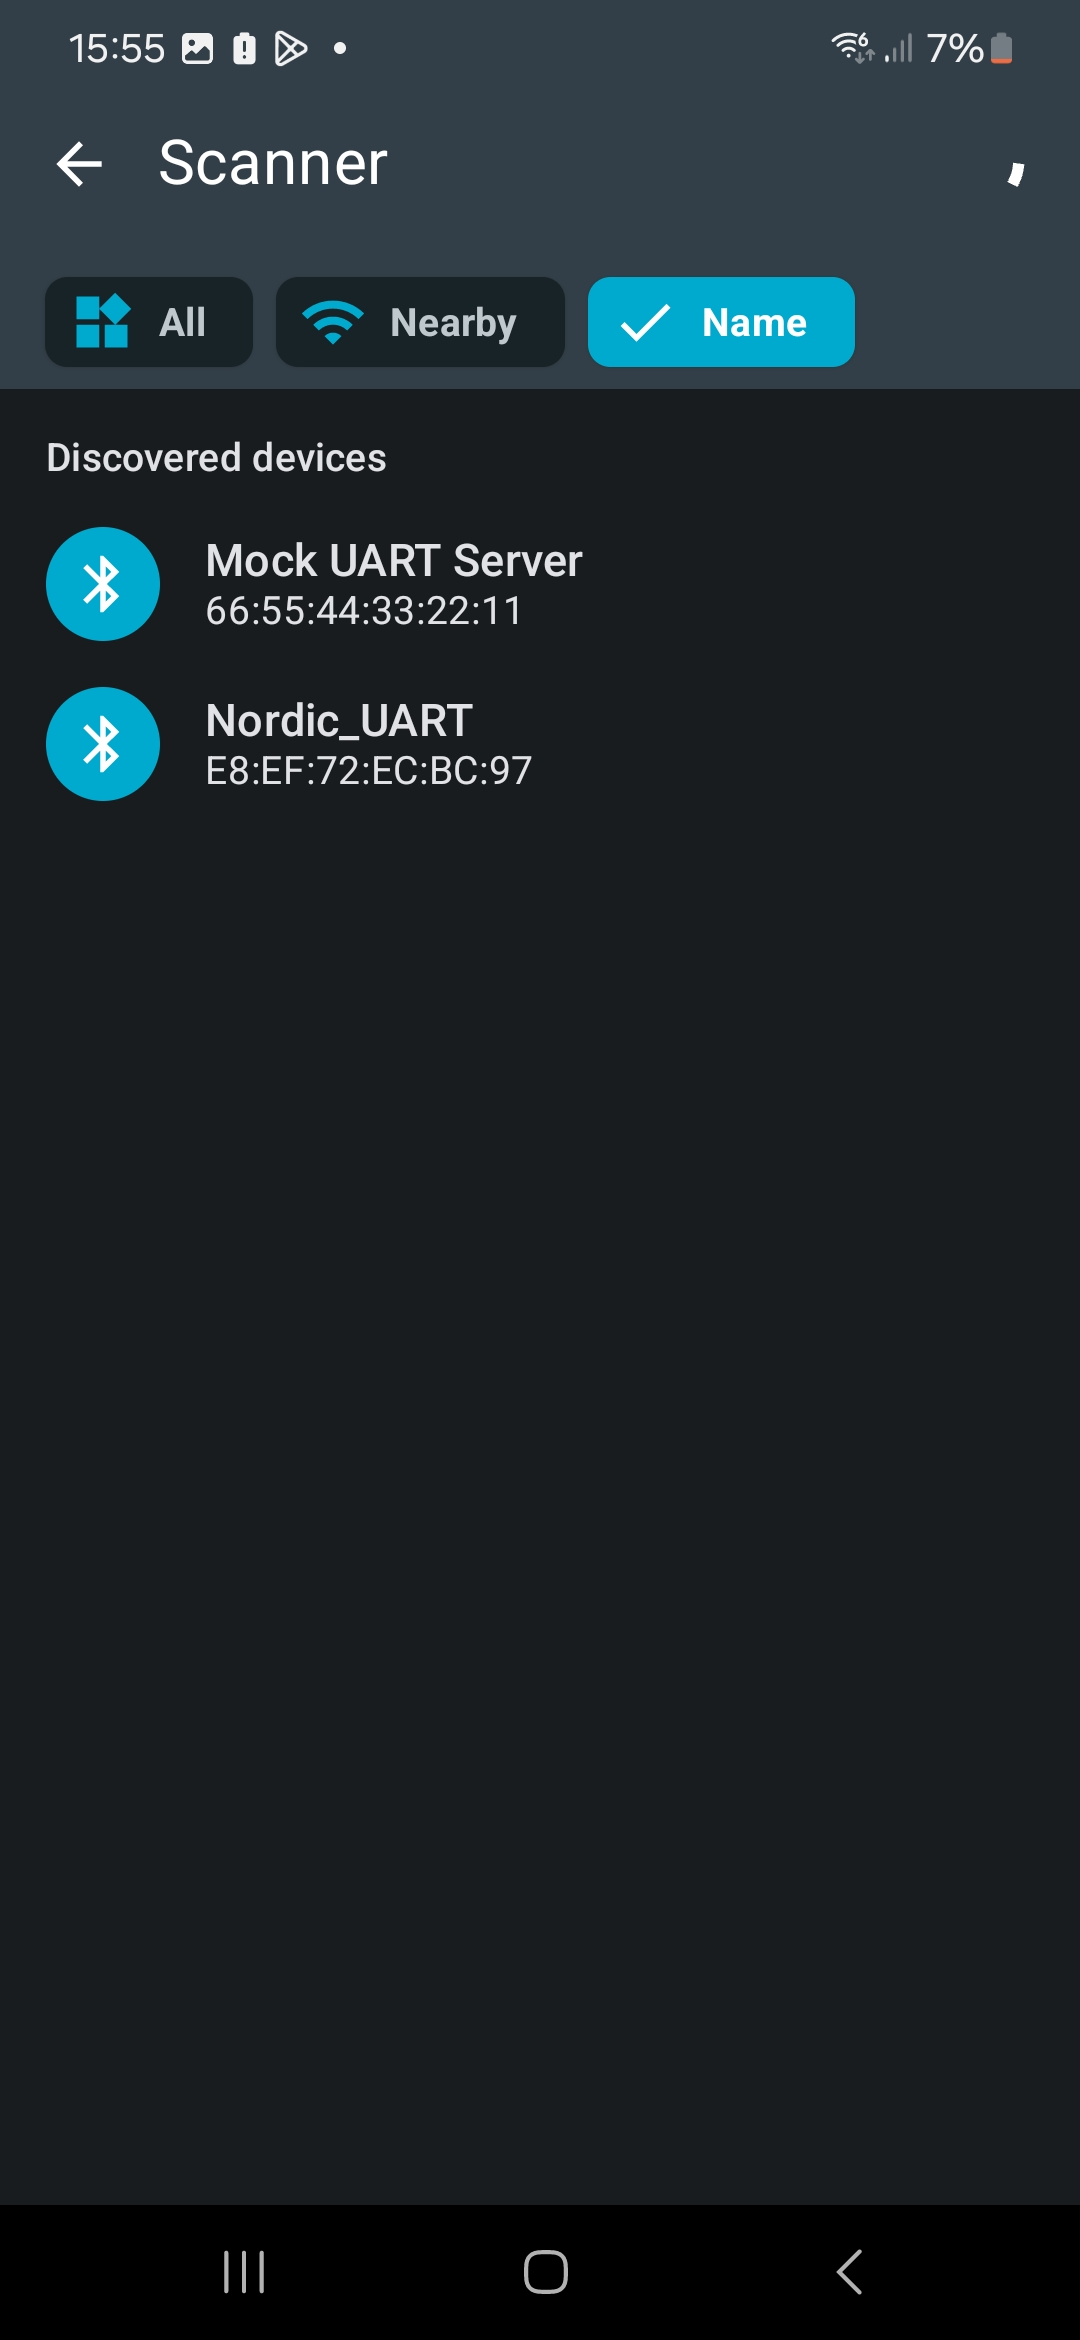
\includegraphics[width=200px]{graphics/nRF_toolbox_connect.jpg}
\label{f:Toolbox_connect}
\end{figure}

\begin{figure}[ht!]
\centering
 \caption{nRF Toolbox UART module screen}
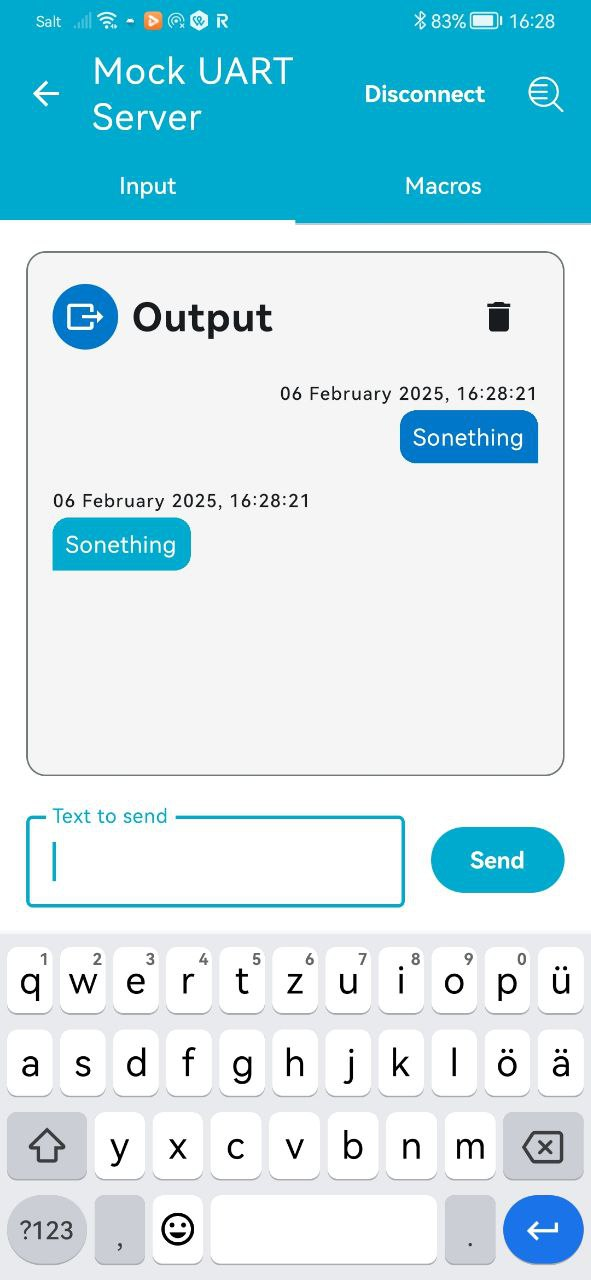
\includegraphics[width=200px]{graphics/nRF_toolbox_messanger.jpg}
\label{f:Toolbox_connect}
\end{figure}

Since the development of an application was not the primary focus of this thesis, it was decided to take the nRF Toolbox app and add a new module for art-traking to it.
The UART module searved as the basis for this new module, since it had a lot of usefull services already implemented.
As with the UART module the art-tracking module opens up the same connection page \ref{f:Toolbox_connect}, that allows the user to select the art-tracking and connect to it.

Once connected, the observation screen is shown (figure \ref{f:Toolbox_art_tracking_empty}).
At the bottom seven parameters can be set: \textit{time}, \textit{max Temp}, \textit{min Temp}, \textit{max Hum}, \textit{min Hum}, \textit{max Angle}, \textit{max Dist}.
The parameters \textit{max}/\textit{min} \textit{Temp}/\textit{Hum} represent the expected range of humidity and temperature.
Any measurement outside these parameter will be considered a dangerous value by the app.
The tollerated difference in angle compared to the previous measurement is set by \textit{max Angle}, larger differences are considered dangerous values.
Distance measurement work analogously with \textit{max Dist} in meters.
The \textit{time} set defines the time that passes enbetween measurements in seconds.
The default is set to 350 seconds.
This means that the time that passes between, for example, the temperature measurements on tag 2 are 350 seconds.


\begin{figure}[ht!]
\centering
 \caption{Art Tracking module oberservation screen before measurements}
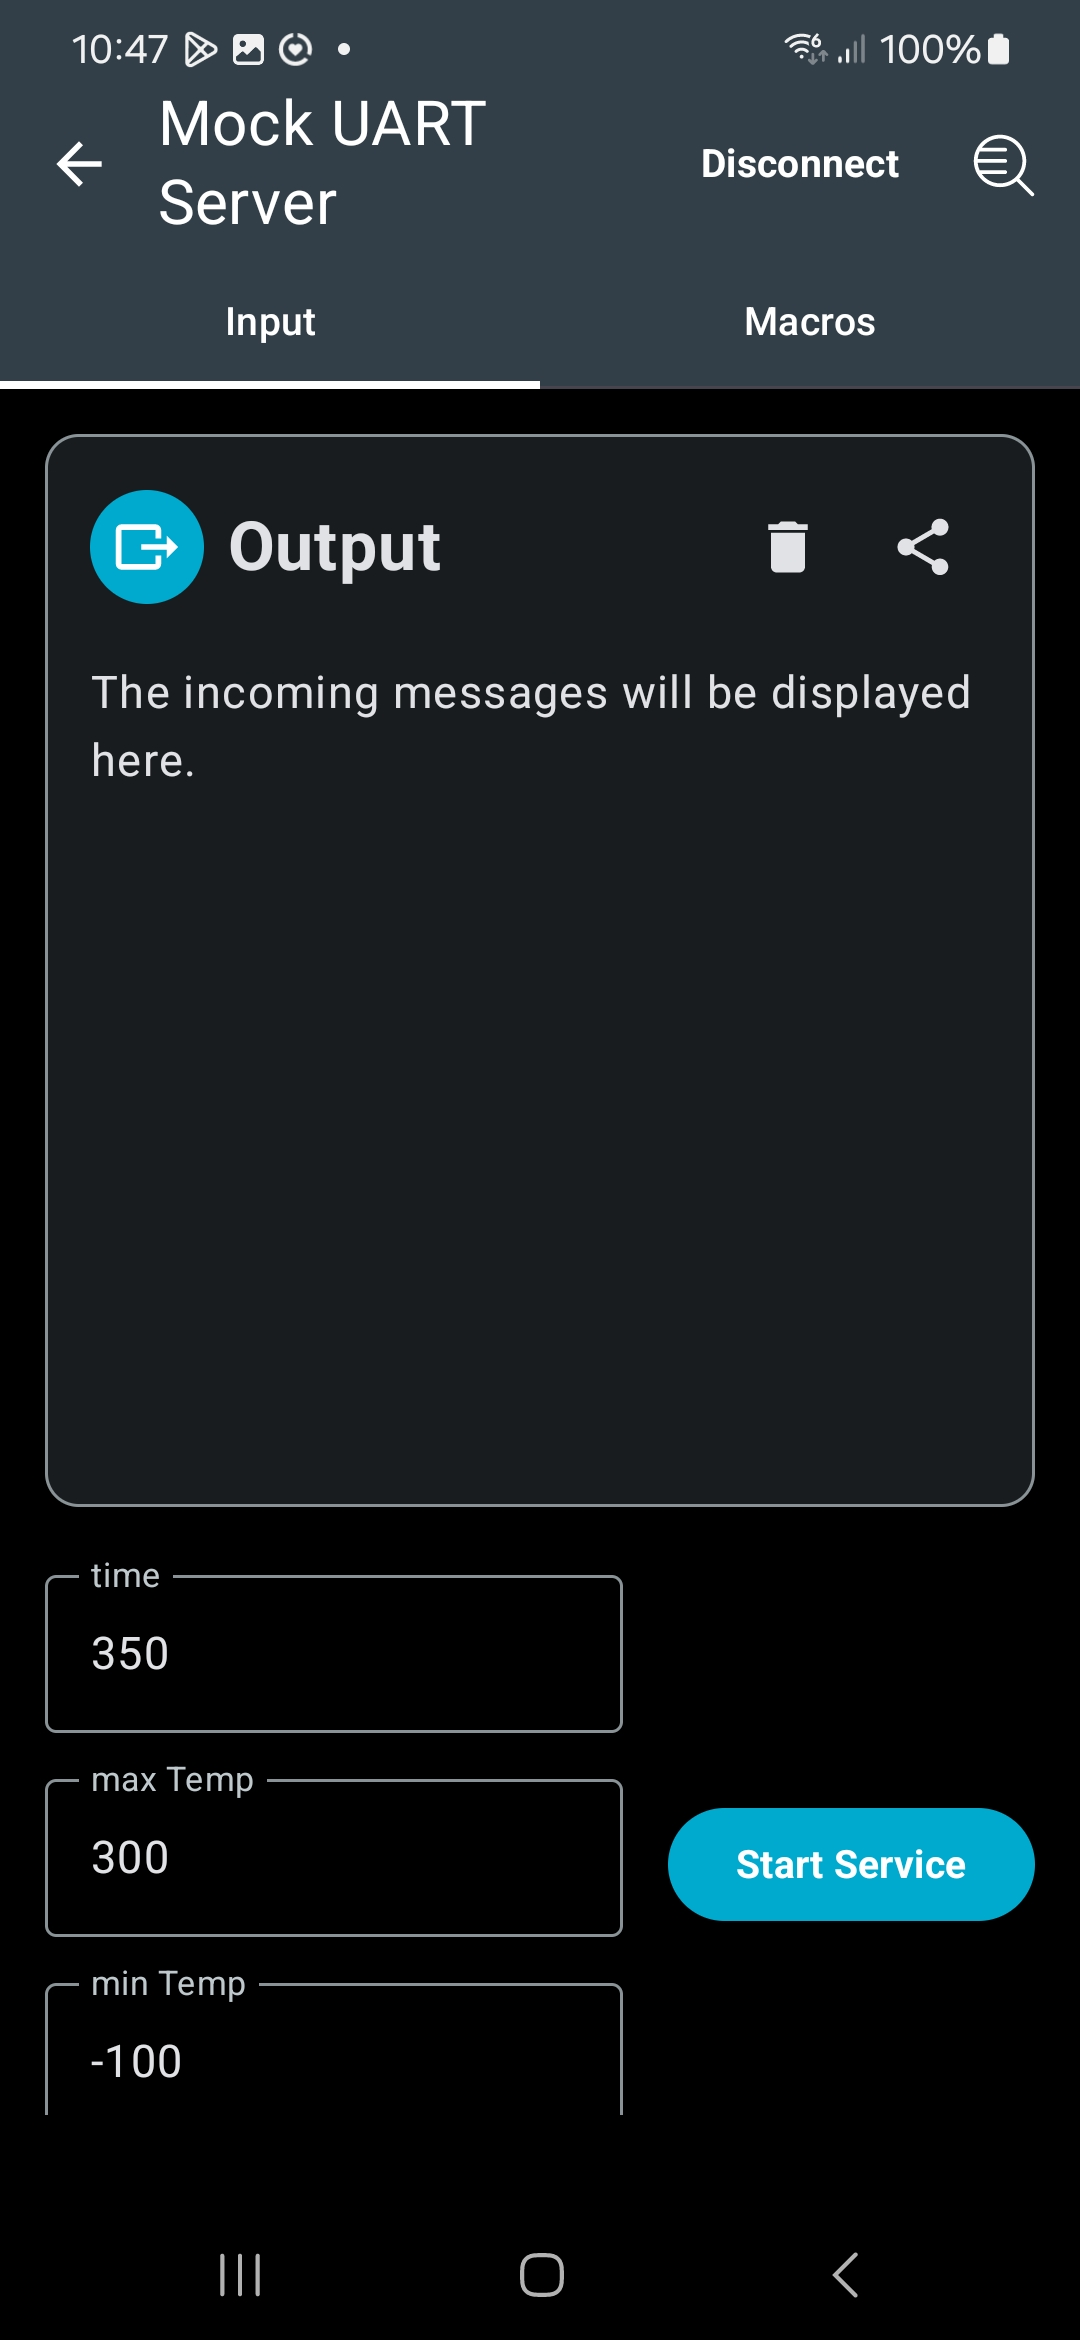
\includegraphics[width=200px]{graphics/nRF_toolbox_art_tracking_empty.jpg}
\label{f:Toolbox_art_tracking_empty}
\end{figure}


When the user presses the \textit{Start Service} button, a services starts that poeriodically queries the tags for the Measurements.
Figure \ref{code:App_main_loop} shows the measurement loop.
Each sensor is assigned a character.
\textit{T} for temperature and humidity, \textit{G} for gyro and \textit{D} for distance.
Each tag has a number, here from one to four since four tags were used in the experiments.
The loop concatenates these two characters and sends the resulting query to the connected tag.
Then the next tag-number is prepared for the next query.
Once all tags have been queried for a sensor, the tag-number starts with the first again and the next sensor is queried.
In between cals the app waits.
The call time for distance-measurement is fixed at 80 seconds.
Distance measurement takes longer than the other sensors, since for every devices three measurements need tobe conducted.
Additionaly the sensors that do not participate in a ranging session are sleeping for a quite generous amount of time, to ensure they don't distrub the ranging session.
80 seconds has been chosen, since it allows enough time for all the ranging to happen, plus two repeats per sensor in case the ranging session fails.
For the other sensors the waiting time in between queries is calculated from the remaining set time, after the ranging time is deducted.

\begin{figure}[h]
    \centering
    \begin{lstlisting}[language=Java]
    private val sensors = listOf("T", "G", "D")
    private val devices = listOf("1", "2", "3", "4")
    private var measurement_type = 0
    private var tag = 0
    private var timeBetweenCals: Long = 3750

    private val runnable = object : Runnable {
        override fun run() {
            if (tag >= list2.size) {
                tag = 0
                measurement_type += 1
            }
            if (measurement_type >= list1.size) {
                measurement_type = 0
            }
            val textToSend = "${list1[measurement_type]}${list2[tag]}"
            artRepository.sendText(textToSend, MacroEol.LF)
            tag += 1
            if(list1[measurement_type] == "D"){
                handler.postDelayed(this, 80000)
            } else {
                handler.postDelayed(this, timeBetweenCals)
            }
        }
    }
    \end{lstlisting}
    % Optionally, add a caption to the figure
    \caption{Section from the ArtMetricService.kt, main measurement loop}
	\label{code:App_main_loop}
\end{figure}

Once the process has started, the queries will appear in the chat window on the right side of the screen.
The responses are on the right side, see figure \ref{code:App_main_loop}.
If the response is inside the set parameters, the message bubble will appear blue.
If the measured value is considered a dangerous value, the text bubble will appear red (see figure \ref{f:Toolbox_art_filled}).
Since the message display is programmed in a asynchronus way, it can happen, that the answer to a query appears before the querry itself, if the querried tag is the same as the connected tag.
The service can be stopped by pressing the \textit{start service} button again or by exiting this screen in any way.


\begin{figure}[ht!]
\centering
 \caption{Art Tracking module, queries and responses}
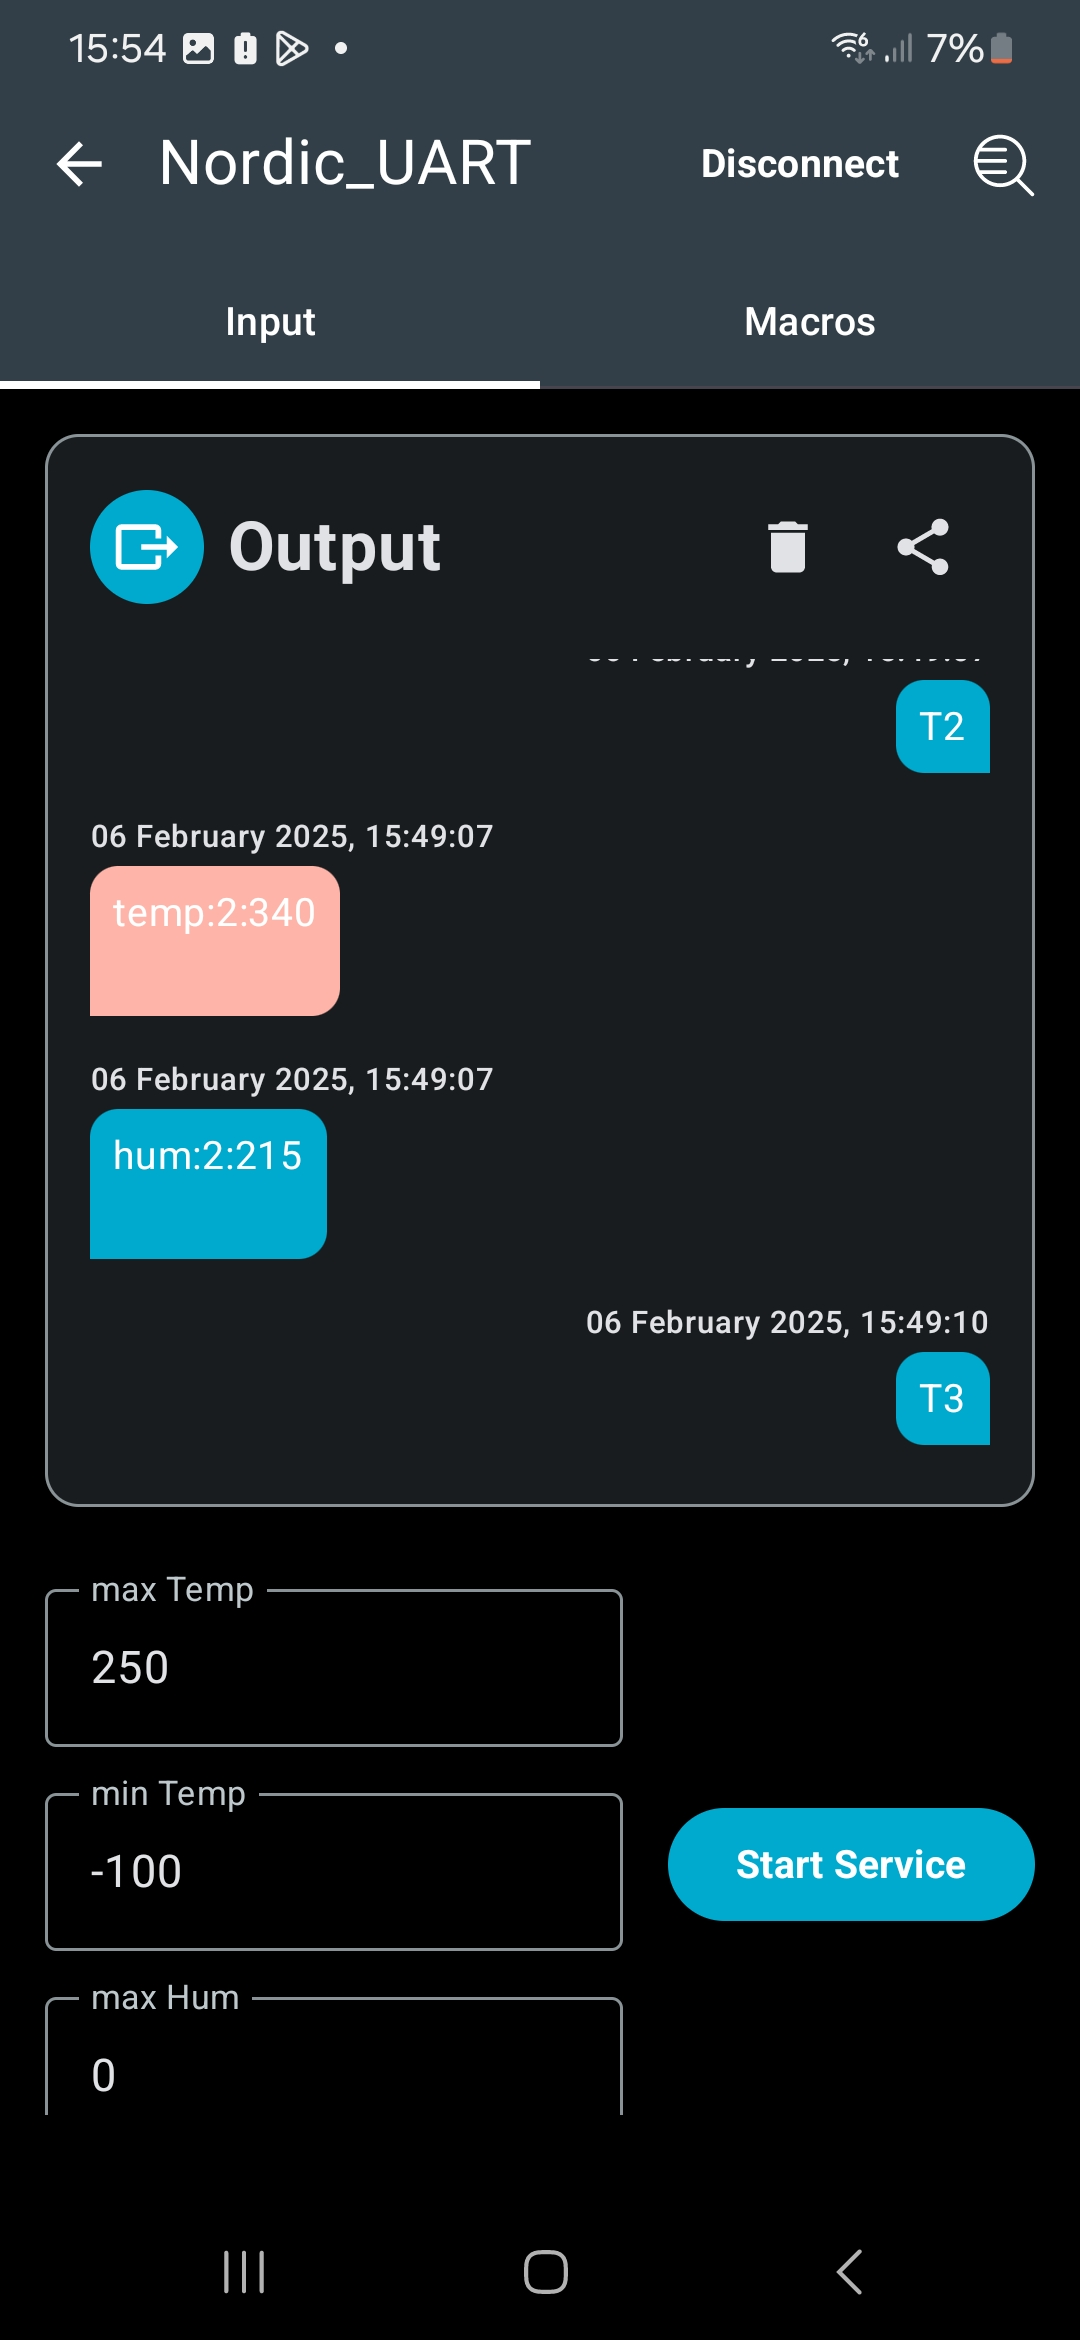
\includegraphics[width=200px]{graphics/nRF_toolbox_Bad_Value_2.jpg}
\label{f:Toolbox_art_filled}
\end{figure}


%TODO: add image that shows an example file
The query-answers are appended to a file that is safed in the app-storage.
The information appendded consits of: the queried tag, the returned values, a timestamp and if the value was unproblematic.
This functionality is intended for experimental evaluation. 
In a real word application, this data should be periodically backed up on a server in a compressed manner.
When pressing the share-button on the top right of the message-box \ref{f:Toolbox_art_filled}.
It will open the Android naitive share functionality, to share the file over mail, an installed messanger, save it to onedrive or send it over Bluetooth.
In this project all files were sent with email.
Pressing the trashcan next to it will delete the chat and empty the file.
This allows the user to distinguish between different testing session.